
%=============================================================================
\section{Introduction}
\label{sec:ddg4-user-manual-introduction}
%=============================================================================
\noindent
This manual should introduce to the DDG4 framework. 
One goal of \DDG is to easily configure the simulation applications
capable of simulating the physics response of detector configurations 
as they are used for example in high energy physics experiments.
In such simulation programs the user normally has to define the 
experimental setup in terms of its geometry and in terms of its 
active elements which sample the detector response.

\noindent
The goal of \DDG is to generalize the configuration of a simulation
application to a degree, which does not force users to write code
to test a detector design. At the same time it should of course
be feasible to supply specialized user written modules which are supposed
to seamlessly operate together with standard modules supplied by the toolkit.
Detector-simulation depends strongly on the use of an underlying simulation
toolkit, the most prominent candidate nowadays being Geant4~\cite{bib:geant4}.
\DDhep supports simulation activities with Geant4 providing
an automatic translation mechanism between geometry representations.
The simulation response in the active elements of the detector
is strongly influenced by the technical 
choices and precise simulations depends on the very specific detection techniques.

\noindent
Similar to the aim of \DDhep\cite{bib:DD4hep}, 
where with time a standard palette of detector
components developed by users should become part of the toolkit,
\DDG also hopes to provide a standard palette of components used
to support simulation activities for detector layouts
where detector designers may base the simulation of a planned experiment 
on these predefined components for initial design and optimization 
studies. The longterm vision is to construct simulation applications
writing only new components not yet present i.e. the main work will be to
select the appropriate components from the palette and connect them
to a functional program.

\noindent
This is not a manual to Geant4 nor the basic infrastructure of \DDhep.
It is assumed that this knowledge is present and the typical glossary 
is known.

%=============================================================================
\section{The Geant4 User Interface}
\label{sec:ddg4-user-manual-geant4-interface}
%=============================================================================

\noindent
The Geant4 simulation toolkit~\cite{bib:geant4} implements a very complex
machinery to simulate the energy deposition of particles traversing materials.
To ease its usage for the clients and to shield clients from the complex
internals when actually implementing a simulation applications for a 
given detector design, it provides several user hooks
as shown in Figure~\ref{fig:ddg4-g4runmanager-anatomy}. Each of these hooks 
serves a well specialized purpose, but unfortunately also leads to very 
specialized applications. One aim of \DDG is to formalize these user 
actions so that the invocation at the appropriate time may be purely
data driven.
\begin{figure}[h]
  \begin{center}
    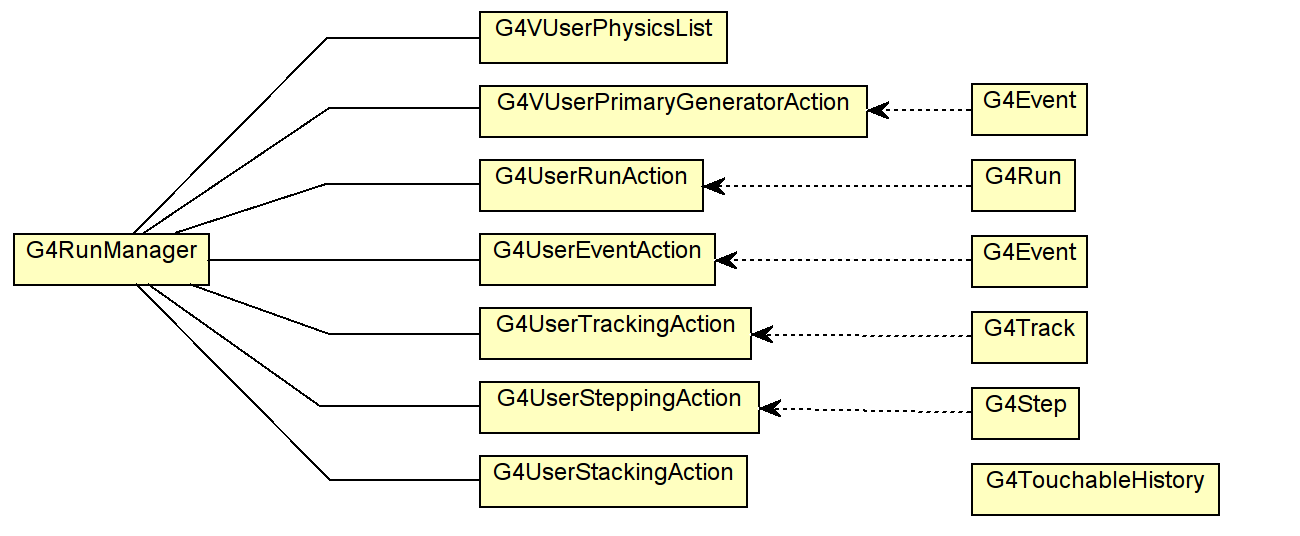
\includegraphics[height=70mm] {DDG4-G4RunManagerAnatomy.png}
    \caption{The various user hooks provided by Geant4. Not shown here
              is the callback system interfacing to the active elements
              of the detector design.}
    \label{fig:ddg4-g4runmanager-anatomy}
  \end{center}
\end{figure}

\noindent
In detail the following object-hooks allow the client to define user provided actions:
\begin{itemize}\itemcompact
\item The \bold{User Physics List} allows the client to customize and define 
    the underlying physics process(es) which define the particle interactions 
    inside the detector defined with the geometry description.
    These interactions define the detector response in terms of 
    energy depositions.
\item The \bold{Run Action} is called once at the start and end of a run. 
    i.e. a series of generated events. These two callbacks
    allow clients to define run-dependent actions such as statistics
    summaries etc.
\item The \bold{Primary Generator Action} is called for every event.
    During the callback all particles are created which form the 
    microscopic kinematic action of the particle collision.
    This input may either origin directly from an event generator program
    or come from file.
\item The \bold{Event Action} is called once at the start and the end of each event.
     It is typically used for a simple analysis of the processed event.
     If the simulated data should be written to some persistent medium, 
     the call at the end of the event processing is the appropriate place.
\item The \bold{Tracking Action} 
\item The \bold{Stepping Action} 
\item The \bold{Stacking Action} 
\end{itemize}
\noindent
Geant4 provides all callbacks with the necessary information in the form of 
appropriate arguments.

\noindent
Besides the callback system, Geant4 provides callbacks whenever a particle
traverses a sensitive volume. These callbacks are called 
- similar to event actions - once at the start and the end of the event,
but in addition, if either the energy deposit of a particle in the 
sensitive volume exceeds some threshold. The callbacks are formalized within 
the base class \tts{G4VSensitiveDetector}.
